


\chapter{Introduction}
\section{Question de recherche}

A partir de données sur le climat, la qualité du sol et les pratiques culturales, est-il possible d’expliquer et de prédire les différents traits de la qualité en bouche des cafés du département de Risaralda ?



\section{Contexte du projet}
Le sujet de ce Travail de Bachelor a été proposé par le « \textit{Centro Internacional de Agricultura Tropical }» (CIAT) qui travaille dans le but d’améliorer la productivité et la gestion de l’agriculture en zone tropicale, et dont les bureaux se trouvent à Cali, en Colombie.\\

À 200 kilomètres de Cali, le comité des caféiculteurs de Risaralda souhaite pouvoir expliquer les différents traits de la qualité en bouche des cafés produits dans les différents secteurs de leur département. La filière café colombienne est en effet en concurrence avec d’autres pays exportateurs sur le marché international, et un des avantages comparatifs de la Colombie est que ses terroirs produisent des cafés de qualité et de caractères affirmés. Il est donc stratégique pour la fédération des caféiculteurs de Colombie d'être en mesure de faire valoir ces spécificités pour aller chercher la valeur ajoutée associée aux produits démarqués du lot.\\


Ce projet a pour but de trouver des méthodes de modélisation afin d’identifier les caractéristiques du café spécifiques à chaque secteur de la région en se basant sur des analyses gustatives, des données climatiques et géographiques, et d’autres données de pratiques culturales.\\


Dans un premier temps, l’objectif est de catégoriser les cafés en tentant de trouver des tendances gustatives par rapport aux conditions de culture. Dans un second temps, il faudra pouvoir prédire la qualité en bouche des cafés par rapport aux conditions environnementales.\\


Le but de cette collaboration sur le long terme est de permettre au département de Risaralda de mettre en valeur la diversité de ses cafés, principalement à des fins de promotion auprès des acheteurs. \\


\section{Contexte des données}
\paragraph{Les données gustatives}sont très relatives aux sens et à la perception de chaque goutteur. Cependant, la SCAA, \textit{Speciality Coffee Association of America}, dispose d’un système de notation basé sur des hypothèses communautaires reconnues ce qui permet d’avoir une certaine régularité dans les données de dégustations. Les cafés sont notés sur 100 points répartis sur plusieurs critères: parfum/arôme, saveur, arrière-goût, acidité, corps, équilibre, douceur, clean-cup (absence de défauts marqués), uniformité et évaluation personnelle du testeur.  Chacun de ces critères est noté sur 10 mais aussi par des termes qualitatifs. Par exemple, la saveur, c’est-à-dire la combinaison de l’odeur et du goût, la première impression qu’on a en goûtant le café, peut être notée 7/10 et “Caramel”. 

\paragraph{Les données climatiques}comprennent les températures maximales, minimales et moyennes, la variation de température pendant la journée (DTR) et les quantités de précipitations. Les moyennes de ces mesures ont été calculée pour chaque mois et extrapolées sur une grande partie du territoire, permettant ainsi d’accéder aux mesures selon l’emplacement désiré à environ 500 mètres près. \\

En prenant par exemple les données de température maximale pour le mois de janvier 2011, en affectant pour chaque valeur une couleur, nous pouvons visualiser les données sous la forme d'une image comme sur la figure \ref{tmax_picture}.


\begin{figure}[h]
	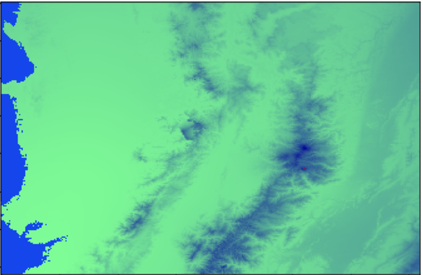
\includegraphics[scale=1]{tmax_picture_1}
	\caption{\label{tmax_picture} Mise sous forme graphique du tableau des température maximales pour le mois de janvier 2011 }
\end{figure}

\paragraph{Les données de qualité de sol}sont subdivisées en profils. Chaque profil est séparé en une ou plusieurs couches d’une certaine profondeur dont sont renseignées les caractéristiques comme le pH, la gravimétrie ou encore le taux de matière organique. 

%TODO
\paragraph{Le système SICA}, pour \textit{Sistema de Información Cafetera}, 


\chapter{Processus de modélisation}
\section{Régression et classification}
La régression est un ensemble de méthodes statistique utilisées afin d'estimer les relations entre des variables, plus précisément entre variables indépendantes (entrées) et dépendantes (sorties). Afin d'estimer les relations entre les variables, des \textit{features} peuvent être extraites comme une moyenne ou la PCA (section \ref{PCAss}) par exemple.\\

La classification, définit simplement le fait de mettre un objet dans une certaine classe ou une autre. 

% https://georgemdallas.wordpress.com/2013/10/30/principal-component-analysis-4-dummies-eigenvectors-eigenvalues-and-dimension-reduction/

% http://mengnote.blogspot.ch/2013/05/an-intuitive-explanation-of-pca.html

% ftp://statgen.ncsu.edu/pub/thorne/molevoclass/AtchleyOct19.pdf

% https://www.analyticsvidhya.com/blog/2015/08/comprehensive-guide-regression/


\subsection{Principal Component Analysis (PCA)}\label{PCAss}
La PCA, pour Analyse en Composante Principale en français, est une méthode qui consiste à transformer un jeu de variables corrélées en nouvelles variables dé-corrélées les unes des autres. Ces nouvelles variables sont appelées composantes principales et permettent de rendre l'information moins redondante. Pour faire plus simple, l'utilité de la Composante Principale est de réduire le nombre de variables tout en gardant un maximum d'information. La figure \ref{PCAdefinition} montre une représentation graphique de la composante principale. 


\begin{figure}[h]
	\caption{\label{PCAdefinition} Description de l'Analyse en Composante Principale. (A) Description d'un objet simple de manière compliquée ( trois dimensions pour par exemple une ellipse en papier) (B) Trouver des nouvelles variables (axes de coordonnées) ortogonaux l'un à l'autre qui pointent dans les directions de la plus grande variance (C) Utiliser les nouvelles variables (axes) pour décrire l'objet d'une manière plus simple. }
	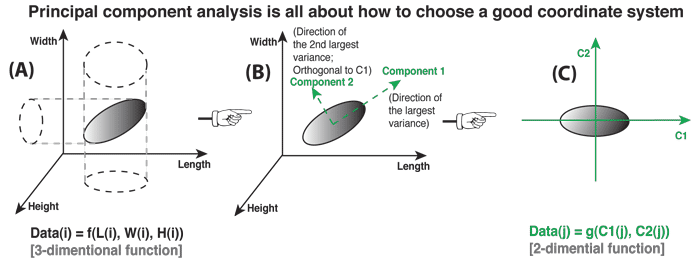
\includegraphics[scale=0.5]{PCA_1}
\end{figure}

\newpage
\subsection{Partial Least Square (PLS)}

% https://www.youtube.com/watch?v=WKEGhyFx0Dg
% https://www.utdallas.edu/~herve/abdi-wireCS-PLS2010.pdf

PLS, originalement pour \textit{Partial Least Squares regression} puis plus récemment pour \textit{Projection to Latent Structures} est une méthode qui combine des propriétés de la PCA ainsi que de multiples régressions linéaires. Au lieu de trouver un hyperplan de la variance maximale, entre les variables dépendantes et indépendantes, cette méthode va trouver un modèle de régression linéaire en projetant les variables indépendantes et dépendantes dans un nouvel espace. Ce sont les variables latentes. Cette méthode est particulièrement utile lorsqu'il est nécessaire de prédire un jeu de variables dépendantes à partir d'un très grand jeu de variables indépendantes. 

\begin{figure}[h]
	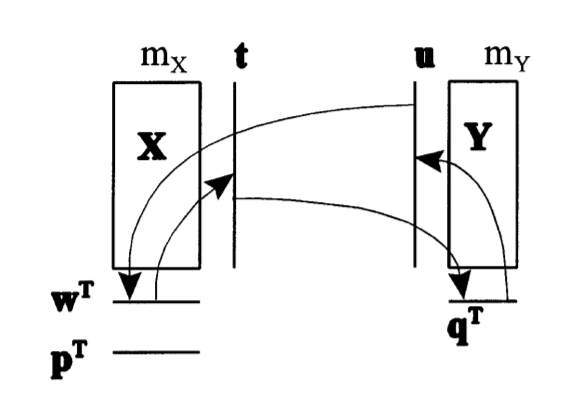
\includegraphics[scale=0.5]{PLS_1}
	\caption{\label{PLSschema}Méthode PLS. X est représenté par son score t et Y par u. Une première estimation de U est multipliée à travers X pour obtenir une aproximation du poid $ \omega_t $. Le poid est normalisé pour être de longueur 1 et remultiplié à travers X pour produire t. A partir de t et de Y, le poid $ q^T $ est obtenu ce qui donne un nouveau vecteur u. Cette opération est répétée jusqu'à la convergence de t.}
	%TODO citer le livre  http://www.umb.no/statisk/specmod/mbseminar/Westerhuis1998.pdf
\end{figure}

\subsection{Multi Block PLS}
% http://www.models.life.ku.dk/~courses/MBtoolbox/pres_IntroMultiBlock.pdf

% https://books.google.ch/books?id=PPUbvBUvmWoC

% http://www.umb.no/statisk/specmod/mbseminar/Westerhuis1998.pdf

La PLS multi block est une extension de la méthode PLS qui sépare les variables indépendantes en plusieurs blocks afin de leur donner une plus grande interpértabilité et plus d'informations sur la structure générale des données. Dans le cadre de ce projet, on peut imaginer séparer les données climatiques des données de sol par exemple.  
L'exécution est très similaire à la méthode PLS classique. 

\begin{figure}[h]
	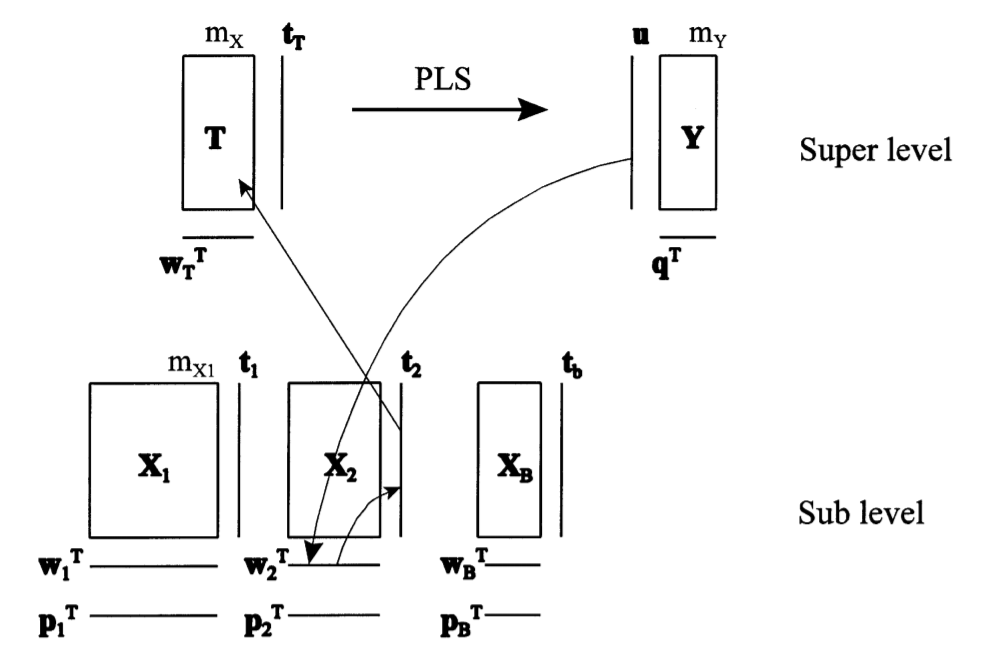
\includegraphics[scale=0.5]{MBPLS_1}
	\caption{\label{MBPLSschema} Méthode MBPLS. Un score de départ u est régressé sur tous les blocs $ X_b $ pour donner les poids variables du bloc $ w^T_b $ Les poids des variables de blocs sont normalisés à la longueur un et multipliés par les blocs pour donner les scores de blocs $ t_b $.  Les scores de blocs sont combinés dans le super bloc T. Un cycle PLS entre T et Y est effectué pour donner le poids superieur $ W^T_T $, qui est également normalisé à la longueur un, et le super score $ t_T $. L'opération est répétée jusqu'à la convergence de $ t_T $. }
	%TODO citer le livre  http://www.umb.no/statisk/specmod/mbseminar/Westerhuis1998.pdf
\end{figure}

\section{Apprentissage supervisé}
% knn, réseaux de neurones etc



\section{Apprentissage non-supervisé}
% som, 






